

\tikzset{every picture/.style={line width=0.75pt}} %set default line width to 0.75pt        

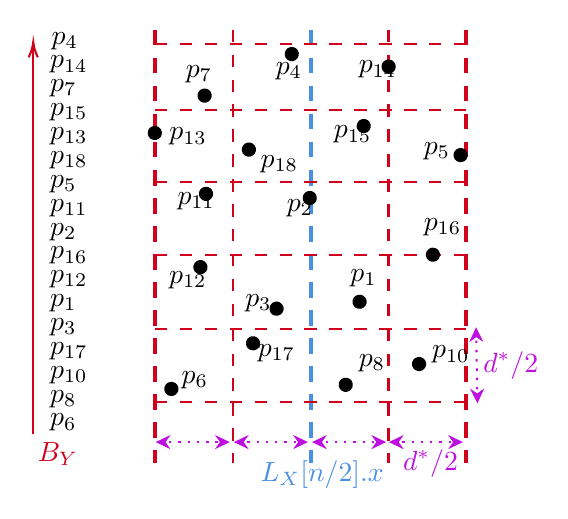
\begin{tikzpicture}[x=0.5pt,y=0.5pt,yscale=-1,xscale=1]
%uncomment if require: \path (0,377); %set diagram left start at 0, and has height of 377

%Straight Lines [id:da6529740224708328] 
\draw [color={rgb, 255:red, 74; green, 144; blue, 226 }  ,draw opacity=1 ][line width=1.5]  [dash pattern={on 5.63pt off 4.5pt}]  (222.5,7) -- (222.5,320) ;
%Straight Lines [id:da3441187372234148] 
\draw [color={rgb, 255:red, 208; green, 2; blue, 27 }  ,draw opacity=1 ][line width=0.75]  [dash pattern={on 4.5pt off 4.5pt}]  (166.25,7) -- (166.25,320) ;
%Straight Lines [id:da06503609524950982] 
\draw [color={rgb, 255:red, 208; green, 2; blue, 27 }  ,draw opacity=1 ][line width=0.75]  [dash pattern={on 4.5pt off 4.5pt}]  (278.75,7) -- (278.75,320) ;
%Straight Lines [id:da01899195473791948] 
\draw [color={rgb, 255:red, 189; green, 16; blue, 224 }  ,draw opacity=1 ] [dash pattern={on 0.84pt off 2.51pt}]  (170,305) -- (217.5,305) ;
\draw [shift={(220.5,305)}, rotate = 180] [fill={rgb, 255:red, 189; green, 16; blue, 224 }  ,fill opacity=1 ][line width=0.08]  [draw opacity=0] (10.72,-5.15) -- (0,0) -- (10.72,5.15) -- (7.12,0) -- cycle    ;
\draw [shift={(167,305)}, rotate = 0] [fill={rgb, 255:red, 189; green, 16; blue, 224 }  ,fill opacity=1 ][line width=0.08]  [draw opacity=0] (10.72,-5.15) -- (0,0) -- (10.72,5.15) -- (7.12,0) -- cycle    ;
%Straight Lines [id:da5930514326113744] 
\draw [color={rgb, 255:red, 189; green, 16; blue, 224 }  ,draw opacity=1 ] [dash pattern={on 0.84pt off 2.51pt}]  (226.5,305) -- (274,305) ;
\draw [shift={(277,305)}, rotate = 180] [fill={rgb, 255:red, 189; green, 16; blue, 224 }  ,fill opacity=1 ][line width=0.08]  [draw opacity=0] (10.72,-5.15) -- (0,0) -- (10.72,5.15) -- (7.12,0) -- cycle    ;
\draw [shift={(223.5,305)}, rotate = 0] [fill={rgb, 255:red, 189; green, 16; blue, 224 }  ,fill opacity=1 ][line width=0.08]  [draw opacity=0] (10.72,-5.15) -- (0,0) -- (10.72,5.15) -- (7.12,0) -- cycle    ;
%Straight Lines [id:da9199871224664768] 
\draw [color={rgb, 255:red, 208; green, 2; blue, 27 }  ,draw opacity=1 ][line width=1.5]  [dash pattern={on 5.63pt off 4.5pt}]  (110,7) -- (110,320) ;
%Straight Lines [id:da313545184348601] 
\draw [color={rgb, 255:red, 208; green, 2; blue, 27 }  ,draw opacity=1 ][line width=1.5]  [dash pattern={on 5.63pt off 4.5pt}]  (335,7) -- (335,320) ;
%Straight Lines [id:da008171567906934074] 
\draw [color={rgb, 255:red, 189; green, 16; blue, 224 }  ,draw opacity=1 ] [dash pattern={on 0.84pt off 2.51pt}]  (113.5,305) -- (161,305) ;
\draw [shift={(164,305)}, rotate = 180] [fill={rgb, 255:red, 189; green, 16; blue, 224 }  ,fill opacity=1 ][line width=0.08]  [draw opacity=0] (10.72,-5.15) -- (0,0) -- (10.72,5.15) -- (7.12,0) -- cycle    ;
\draw [shift={(110.5,305)}, rotate = 0] [fill={rgb, 255:red, 189; green, 16; blue, 224 }  ,fill opacity=1 ][line width=0.08]  [draw opacity=0] (10.72,-5.15) -- (0,0) -- (10.72,5.15) -- (7.12,0) -- cycle    ;
%Straight Lines [id:da5296316037034452] 
\draw [color={rgb, 255:red, 189; green, 16; blue, 224 }  ,draw opacity=1 ] [dash pattern={on 0.84pt off 2.51pt}]  (282,305) -- (329.5,305) ;
\draw [shift={(332.5,305)}, rotate = 180] [fill={rgb, 255:red, 189; green, 16; blue, 224 }  ,fill opacity=1 ][line width=0.08]  [draw opacity=0] (10.72,-5.15) -- (0,0) -- (10.72,5.15) -- (7.12,0) -- cycle    ;
\draw [shift={(279,305)}, rotate = 0] [fill={rgb, 255:red, 189; green, 16; blue, 224 }  ,fill opacity=1 ][line width=0.08]  [draw opacity=0] (10.72,-5.15) -- (0,0) -- (10.72,5.15) -- (7.12,0) -- cycle    ;
%Straight Lines [id:da4429916887913099] 
\draw [color={rgb, 255:red, 208; green, 2; blue, 27 }  ,draw opacity=1 ][line width=0.75]  [dash pattern={on 4.5pt off 4.5pt}]  (110,276) -- (335,276) ;
%Straight Lines [id:da6783093940157634] 
\draw [color={rgb, 255:red, 208; green, 2; blue, 27 }  ,draw opacity=1 ][line width=0.75]  [dash pattern={on 4.5pt off 4.5pt}]  (110,223) -- (335,223) ;
%Straight Lines [id:da3395926668100431] 
\draw [color={rgb, 255:red, 208; green, 2; blue, 27 }  ,draw opacity=1 ][line width=0.75]  [dash pattern={on 4.5pt off 4.5pt}]  (110,170) -- (335,170) ;
%Straight Lines [id:da11772188438625031] 
\draw [color={rgb, 255:red, 208; green, 2; blue, 27 }  ,draw opacity=1 ][line width=0.75]  [dash pattern={on 4.5pt off 4.5pt}]  (110,117) -- (335,117) ;
%Straight Lines [id:da5874985603564619] 
\draw [color={rgb, 255:red, 208; green, 2; blue, 27 }  ,draw opacity=1 ][line width=0.75]  [dash pattern={on 4.5pt off 4.5pt}]  (110,65) -- (335,65) ;
%Straight Lines [id:da706623823441126] 
\draw [color={rgb, 255:red, 208; green, 2; blue, 27 }  ,draw opacity=1 ][line width=0.75]  [dash pattern={on 4.5pt off 4.5pt}]  (110,17) -- (335,17) ;
%Straight Lines [id:da8387514930702964] 
\draw [color={rgb, 255:red, 189; green, 16; blue, 224 }  ,draw opacity=1 ] [dash pattern={on 0.84pt off 2.51pt}]  (342.05,225) -- (342.95,274) ;
\draw [shift={(343,277)}, rotate = 268.96] [fill={rgb, 255:red, 189; green, 16; blue, 224 }  ,fill opacity=1 ][line width=0.08]  [draw opacity=0] (10.72,-5.15) -- (0,0) -- (10.72,5.15) -- (7.12,0) -- cycle    ;
\draw [shift={(342,222)}, rotate = 88.96] [fill={rgb, 255:red, 189; green, 16; blue, 224 }  ,fill opacity=1 ][line width=0.08]  [draw opacity=0] (10.72,-5.15) -- (0,0) -- (10.72,5.15) -- (7.12,0) -- cycle    ;
%Flowchart: Connector [id:dp8923414673582244] 
\draw  [fill={rgb, 255:red, 0; green, 0; blue, 0 }  ,fill opacity=1 ] (248.64,267.88) .. controls (246.27,268.34) and (243.98,266.78) .. (243.52,264.41) .. controls (243.07,262.03) and (244.63,259.74) .. (247,259.29) .. controls (249.37,258.83) and (251.67,260.39) .. (252.12,262.77) .. controls (252.57,265.14) and (251.02,267.43) .. (248.64,267.88) -- cycle ;
%Flowchart: Connector [id:dp6825138981911604] 
\draw  [fill={rgb, 255:red, 0; green, 0; blue, 0 }  ,fill opacity=1 ] (181.64,237.88) .. controls (179.27,238.34) and (176.98,236.78) .. (176.52,234.41) .. controls (176.07,232.03) and (177.63,229.74) .. (180,229.29) .. controls (182.37,228.83) and (184.67,230.39) .. (185.12,232.77) .. controls (185.57,235.14) and (184.02,237.43) .. (181.64,237.88) -- cycle ;
%Flowchart: Connector [id:dp4157984407010722] 
\draw  [fill={rgb, 255:red, 0; green, 0; blue, 0 }  ,fill opacity=1 ] (122.64,270.88) .. controls (120.27,271.34) and (117.98,269.78) .. (117.52,267.41) .. controls (117.07,265.03) and (118.63,262.74) .. (121,262.29) .. controls (123.37,261.83) and (125.67,263.39) .. (126.12,265.77) .. controls (126.57,268.14) and (125.02,270.43) .. (122.64,270.88) -- cycle ;
%Flowchart: Connector [id:dp8333199543319949] 
\draw  [fill={rgb, 255:red, 0; green, 0; blue, 0 }  ,fill opacity=1 ] (301.64,252.88) .. controls (299.27,253.34) and (296.98,251.78) .. (296.52,249.41) .. controls (296.07,247.03) and (297.63,244.74) .. (300,244.29) .. controls (302.37,243.83) and (304.67,245.39) .. (305.12,247.77) .. controls (305.57,250.14) and (304.02,252.43) .. (301.64,252.88) -- cycle ;
%Flowchart: Connector [id:dp36334472410839813] 
\draw  [fill={rgb, 255:red, 0; green, 0; blue, 0 }  ,fill opacity=1 ] (258.64,207.88) .. controls (256.27,208.34) and (253.98,206.78) .. (253.52,204.41) .. controls (253.07,202.03) and (254.63,199.74) .. (257,199.29) .. controls (259.37,198.83) and (261.67,200.39) .. (262.12,202.77) .. controls (262.57,205.14) and (261.02,207.43) .. (258.64,207.88) -- cycle ;
%Flowchart: Connector [id:dp09374517288306172] 
\draw  [fill={rgb, 255:red, 0; green, 0; blue, 0 }  ,fill opacity=1 ] (198.64,212.88) .. controls (196.27,213.34) and (193.98,211.78) .. (193.52,209.41) .. controls (193.07,207.03) and (194.63,204.74) .. (197,204.29) .. controls (199.37,203.83) and (201.67,205.39) .. (202.12,207.77) .. controls (202.57,210.14) and (201.02,212.43) .. (198.64,212.88) -- cycle ;
%Flowchart: Connector [id:dp2674555355524125] 
\draw  [fill={rgb, 255:red, 0; green, 0; blue, 0 }  ,fill opacity=1 ] (143.64,182.88) .. controls (141.27,183.34) and (138.98,181.78) .. (138.52,179.41) .. controls (138.07,177.03) and (139.63,174.74) .. (142,174.29) .. controls (144.37,173.83) and (146.67,175.39) .. (147.12,177.77) .. controls (147.57,180.14) and (146.02,182.43) .. (143.64,182.88) -- cycle ;
%Flowchart: Connector [id:dp4988189914468546] 
\draw  [fill={rgb, 255:red, 0; green, 0; blue, 0 }  ,fill opacity=1 ] (311.64,173.88) .. controls (309.27,174.34) and (306.98,172.78) .. (306.52,170.41) .. controls (306.07,168.03) and (307.63,165.74) .. (310,165.29) .. controls (312.37,164.83) and (314.67,166.39) .. (315.12,168.77) .. controls (315.57,171.14) and (314.02,173.43) .. (311.64,173.88) -- cycle ;
%Flowchart: Connector [id:dp6877256898622583] 
\draw  [fill={rgb, 255:red, 0; green, 0; blue, 0 }  ,fill opacity=1 ] (222.64,132.88) .. controls (220.27,133.34) and (217.98,131.78) .. (217.52,129.41) .. controls (217.07,127.03) and (218.63,124.74) .. (221,124.29) .. controls (223.37,123.83) and (225.67,125.39) .. (226.12,127.77) .. controls (226.57,130.14) and (225.02,132.43) .. (222.64,132.88) -- cycle ;
%Flowchart: Connector [id:dp7258428027313548] 
\draw  [fill={rgb, 255:red, 0; green, 0; blue, 0 }  ,fill opacity=1 ] (147.64,129.88) .. controls (145.27,130.34) and (142.98,128.78) .. (142.52,126.41) .. controls (142.07,124.03) and (143.63,121.74) .. (146,121.29) .. controls (148.37,120.83) and (150.67,122.39) .. (151.12,124.77) .. controls (151.57,127.14) and (150.02,129.43) .. (147.64,129.88) -- cycle ;
%Flowchart: Connector [id:dp4759673781795757] 
\draw  [fill={rgb, 255:red, 0; green, 0; blue, 0 }  ,fill opacity=1 ] (331.64,101.88) .. controls (329.27,102.34) and (326.98,100.78) .. (326.52,98.41) .. controls (326.07,96.03) and (327.63,93.74) .. (330,93.29) .. controls (332.37,92.83) and (334.67,94.39) .. (335.12,96.77) .. controls (335.57,99.14) and (334.02,101.43) .. (331.64,101.88) -- cycle ;
%Flowchart: Connector [id:dp8213326726444833] 
\draw  [fill={rgb, 255:red, 0; green, 0; blue, 0 }  ,fill opacity=1 ] (261.64,80.88) .. controls (259.27,81.34) and (256.98,79.78) .. (256.52,77.41) .. controls (256.07,75.03) and (257.63,72.74) .. (260,72.29) .. controls (262.37,71.83) and (264.67,73.39) .. (265.12,75.77) .. controls (265.57,78.14) and (264.02,80.43) .. (261.64,80.88) -- cycle ;
%Flowchart: Connector [id:dp19921591820820672] 
\draw  [fill={rgb, 255:red, 0; green, 0; blue, 0 }  ,fill opacity=1 ] (178.64,97.88) .. controls (176.27,98.34) and (173.98,96.78) .. (173.52,94.41) .. controls (173.07,92.03) and (174.63,89.74) .. (177,89.29) .. controls (179.37,88.83) and (181.67,90.39) .. (182.12,92.77) .. controls (182.57,95.14) and (181.02,97.43) .. (178.64,97.88) -- cycle ;
%Flowchart: Connector [id:dp45521771767073826] 
\draw  [fill={rgb, 255:red, 0; green, 0; blue, 0 }  ,fill opacity=1 ] (110.64,85.88) .. controls (108.27,86.34) and (105.98,84.78) .. (105.52,82.41) .. controls (105.07,80.03) and (106.63,77.74) .. (109,77.29) .. controls (111.37,76.83) and (113.67,78.39) .. (114.12,80.77) .. controls (114.57,83.14) and (113.02,85.43) .. (110.64,85.88) -- cycle ;
%Flowchart: Connector [id:dp6969160770264389] 
\draw  [fill={rgb, 255:red, 0; green, 0; blue, 0 }  ,fill opacity=1 ] (279.64,37.88) .. controls (277.27,38.34) and (274.98,36.78) .. (274.52,34.41) .. controls (274.07,32.03) and (275.63,29.74) .. (278,29.29) .. controls (280.37,28.83) and (282.67,30.39) .. (283.12,32.77) .. controls (283.57,35.14) and (282.02,37.43) .. (279.64,37.88) -- cycle ;
%Flowchart: Connector [id:dp17503792181776967] 
\draw  [fill={rgb, 255:red, 0; green, 0; blue, 0 }  ,fill opacity=1 ] (209.64,28.88) .. controls (207.27,29.34) and (204.98,27.78) .. (204.52,25.41) .. controls (204.07,23.03) and (205.63,20.74) .. (208,20.29) .. controls (210.37,19.83) and (212.67,21.39) .. (213.12,23.77) .. controls (213.57,26.14) and (212.02,28.43) .. (209.64,28.88) -- cycle ;
%Flowchart: Connector [id:dp7711561658315957] 
\draw  [fill={rgb, 255:red, 0; green, 0; blue, 0 }  ,fill opacity=1 ] (146.64,58.88) .. controls (144.27,59.34) and (141.98,57.78) .. (141.52,55.41) .. controls (141.07,53.03) and (142.63,50.74) .. (145,50.29) .. controls (147.37,49.83) and (149.67,51.39) .. (150.12,53.77) .. controls (150.57,56.14) and (149.02,58.43) .. (146.64,58.88) -- cycle ;
%Straight Lines [id:da023124782613843764] 
\draw [color={rgb, 255:red, 208; green, 2; blue, 27 }  ,draw opacity=1 ]   (22,299) -- (22,18) ;
\draw [shift={(22,16)}, rotate = 90] [color={rgb, 255:red, 208; green, 2; blue, 27 }  ,draw opacity=1 ][line width=0.75]    (10.93,-3.29) .. controls (6.95,-1.4) and (3.31,-0.3) .. (0,0) .. controls (3.31,0.3) and (6.95,1.4) .. (10.93,3.29)   ;

% Text Node
\draw (184,316.45) node [anchor=north west][inner sep=0.75pt]  [color={rgb, 255:red, 74; green, 144; blue, 226 }  ,opacity=1 ] [align=left] {$\displaystyle L_{X}[ n/2] .x$};
% Text Node
\draw (287,308.41) node [anchor=north west][inner sep=0.75pt]  [color={rgb, 255:red, 189; green, 16; blue, 224 }  ,opacity=1 ] [align=left] {$\displaystyle d^{*} /2$};
% Text Node
\draw (345,237.41) node [anchor=north west][inner sep=0.75pt]  [color={rgb, 255:red, 189; green, 16; blue, 224 }  ,opacity=1 ] [align=left] {$\displaystyle d^{*} /2$};
% Text Node
\draw (127,251.45) node [anchor=north west][inner sep=0.75pt]   [align=left] {$\displaystyle p_{6}$};
% Text Node
\draw (182,232.29) node [anchor=north west][inner sep=0.75pt]   [align=left] {$\displaystyle p_{17}$};
% Text Node
\draw (255,239.29) node [anchor=north west][inner sep=0.75pt]   [align=left] {$\displaystyle p_{8}$};
% Text Node
\draw (308,233.29) node [anchor=north west][inner sep=0.75pt]   [align=left] {$\displaystyle p_{10}$};
% Text Node
\draw (249,178.29) node [anchor=north west][inner sep=0.75pt]   [align=left] {$\displaystyle p_{1}$};
% Text Node
\draw (173,196.29) node [anchor=north west][inner sep=0.75pt]   [align=left] {$\displaystyle p_{3}$};
% Text Node
\draw (118,179.29) node [anchor=north west][inner sep=0.75pt]   [align=left] {$\displaystyle p_{12}$};
% Text Node
\draw (124,122.29) node [anchor=north west][inner sep=0.75pt]   [align=left] {$\displaystyle p_{11}$};
% Text Node
\draw (203,127.29) node [anchor=north west][inner sep=0.75pt]   [align=left] {$\displaystyle p_{2}$};
% Text Node
\draw (237,74.29) node [anchor=north west][inner sep=0.75pt]   [align=left] {$\displaystyle p_{15}$};
% Text Node
\draw (302,86.29) node [anchor=north west][inner sep=0.75pt]   [align=left] {$\displaystyle p_{5}$};
% Text Node
\draw (255,27.29) node [anchor=north west][inner sep=0.75pt]   [align=left] {$\displaystyle p_{14}$};
% Text Node
\draw (195,28.29) node [anchor=north west][inner sep=0.75pt]   [align=left] {$\displaystyle p_{4}$};
% Text Node
\draw (130,30.29) node [anchor=north west][inner sep=0.75pt]   [align=left] {$\displaystyle p_{7}$};
% Text Node
\draw (184.12,95.77) node [anchor=north west][inner sep=0.75pt]   [align=left] {$\displaystyle p_{18}$};
% Text Node
\draw (118.12,75.77) node [anchor=north west][inner sep=0.75pt]   [align=left] {$\displaystyle p_{13}$};
% Text Node
\draw (302,141.29) node [anchor=north west][inner sep=0.75pt]   [align=left] {$\displaystyle p_{16}$};
% Text Node
\draw (32,282.45) node [anchor=north west][inner sep=0.75pt]   [align=left] {$\displaystyle p_{6}$};
% Text Node
\draw (32,230.73) node [anchor=north west][inner sep=0.75pt]   [align=left] {$\displaystyle p_{17}$};
% Text Node
\draw (32,265.23) node [anchor=north west][inner sep=0.75pt]   [align=left] {$\displaystyle p_{8}$};
% Text Node
\draw (32,247.98) node [anchor=north west][inner sep=0.75pt]   [align=left] {$\displaystyle p_{10}$};
% Text Node
\draw (32,196.23) node [anchor=north west][inner sep=0.75pt]   [align=left] {$\displaystyle p_{1}$};
% Text Node
\draw (32,213.48) node [anchor=north west][inner sep=0.75pt]   [align=left] {$\displaystyle p_{3}$};
% Text Node
\draw (32,178.98) node [anchor=north west][inner sep=0.75pt]   [align=left] {$\displaystyle p_{12}$};
% Text Node
\draw (32,127.23) node [anchor=north west][inner sep=0.75pt]   [align=left] {$\displaystyle p_{11}$};
% Text Node
\draw (32,144.48) node [anchor=north west][inner sep=0.75pt]   [align=left] {$\displaystyle p_{2}$};
% Text Node
\draw (32,58.23) node [anchor=north west][inner sep=0.75pt]   [align=left] {$\displaystyle p_{15}$};
% Text Node
\draw (32,109.98) node [anchor=north west][inner sep=0.75pt]   [align=left] {$\displaystyle p_{5}$};
% Text Node
\draw (32,23.73) node [anchor=north west][inner sep=0.75pt]   [align=left] {$\displaystyle p_{14}$};
% Text Node
\draw (33,6.48) node [anchor=north west][inner sep=0.75pt]   [align=left] {$\displaystyle p_{4}$};
% Text Node
\draw (32,40.98) node [anchor=north west][inner sep=0.75pt]   [align=left] {$\displaystyle p_{7}$};
% Text Node
\draw (32,92.73) node [anchor=north west][inner sep=0.75pt]   [align=left] {$\displaystyle p_{18}$};
% Text Node
\draw (32,75.48) node [anchor=north west][inner sep=0.75pt]   [align=left] {$\displaystyle p_{13}$};
% Text Node
\draw (32,161.73) node [anchor=north west][inner sep=0.75pt]   [align=left] {$\displaystyle p_{16}$};
% Text Node
\draw (23,303) node [anchor=north west][inner sep=0.75pt]  [color={rgb, 255:red, 208; green, 2; blue, 27 }  ,opacity=1 ] [align=left] {$\displaystyle B_{Y}$};


\end{tikzpicture}

